
\documentclass[template=tabling,81pt,headonall]{azmoon}
\usepackage{xepersian}
\usepackage{amsfonts}
\usepackage{graphicx}
\usepackage{svg}
\svgpath{ {./images/} }
\graphicspath{ {./images/} }
\settextfont{Yas}
\setdigitfont{A Iranian Sans}
\usepackage{fontawesome5}

\printanswers
    \teacher{محمد صالح علی اکبری}
    \teachertitle{دبیر}
    \city{گناباد}
    \schooltitle{متوسطه دوره دوم}
    \school{شاهد امام (ره)}
    \grade{دهم}
    \branch{۱۷۱}
    \topic{ریاضی}
    \examdate{17/11/1402}
    \answertime{70 دقیقه}
    \begin{document}
	\begin{questions}
		\nointerlineskip%
		\vskip-\baselineskip
		\question[3]{%
جدول زیر نمایش‌های یک رابطه مشخص شده‌اند. جاهای خالی را پر کنید. \\ 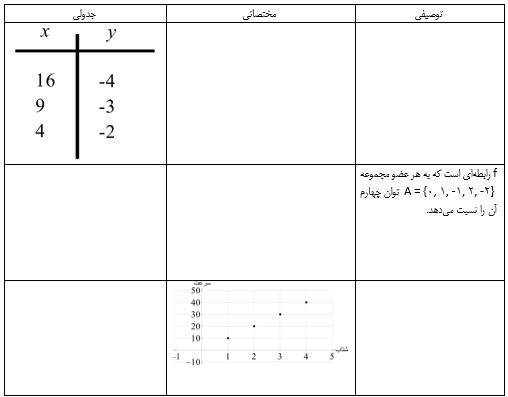
\includegraphics[scale = 1]{Screenshot 2024-02-05 220237}}\question[1.5]{%
اگر رابطه f تابع باشد، در این صورت حاصل $x^2+y^2$ را بدست آورید. \\ $f = {(2,x+y), (2,4), (5,2), (3,4) , (5,x-y)}$‌
\\‌
\\}\question[2]{%
دامنه و برد هر یک از توابع زیر را مشخص کنید.
    \begin{parts}[1]\part{$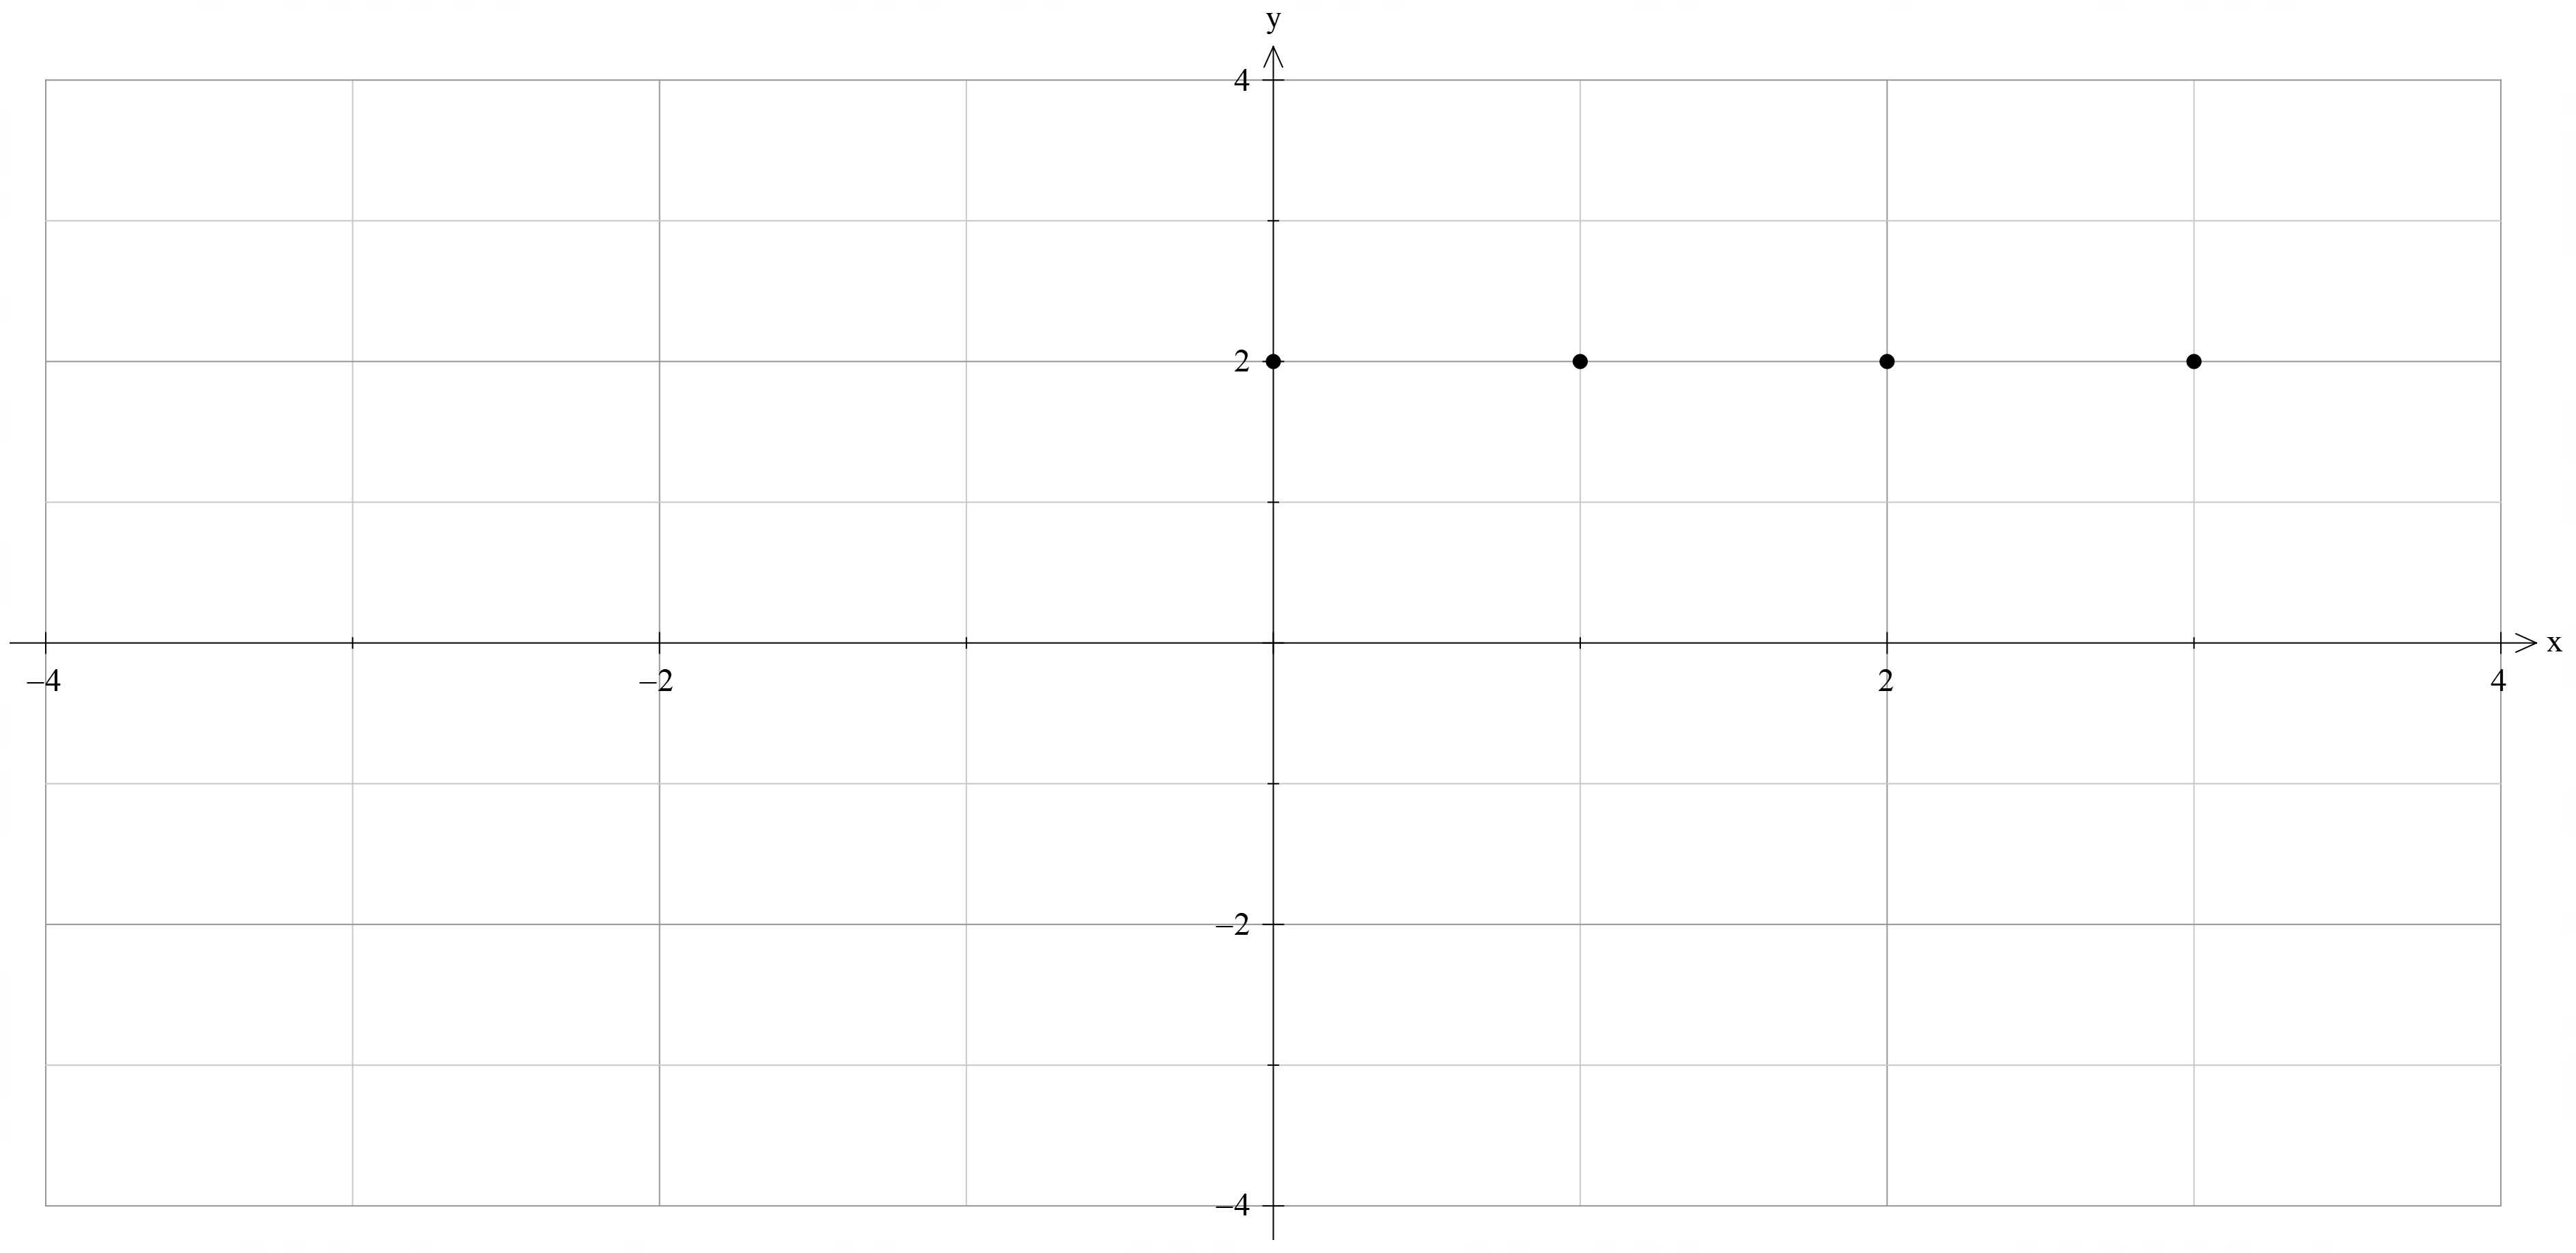
\includegraphics[scale = 0.2]{نمودار_معادله}$}
\part{$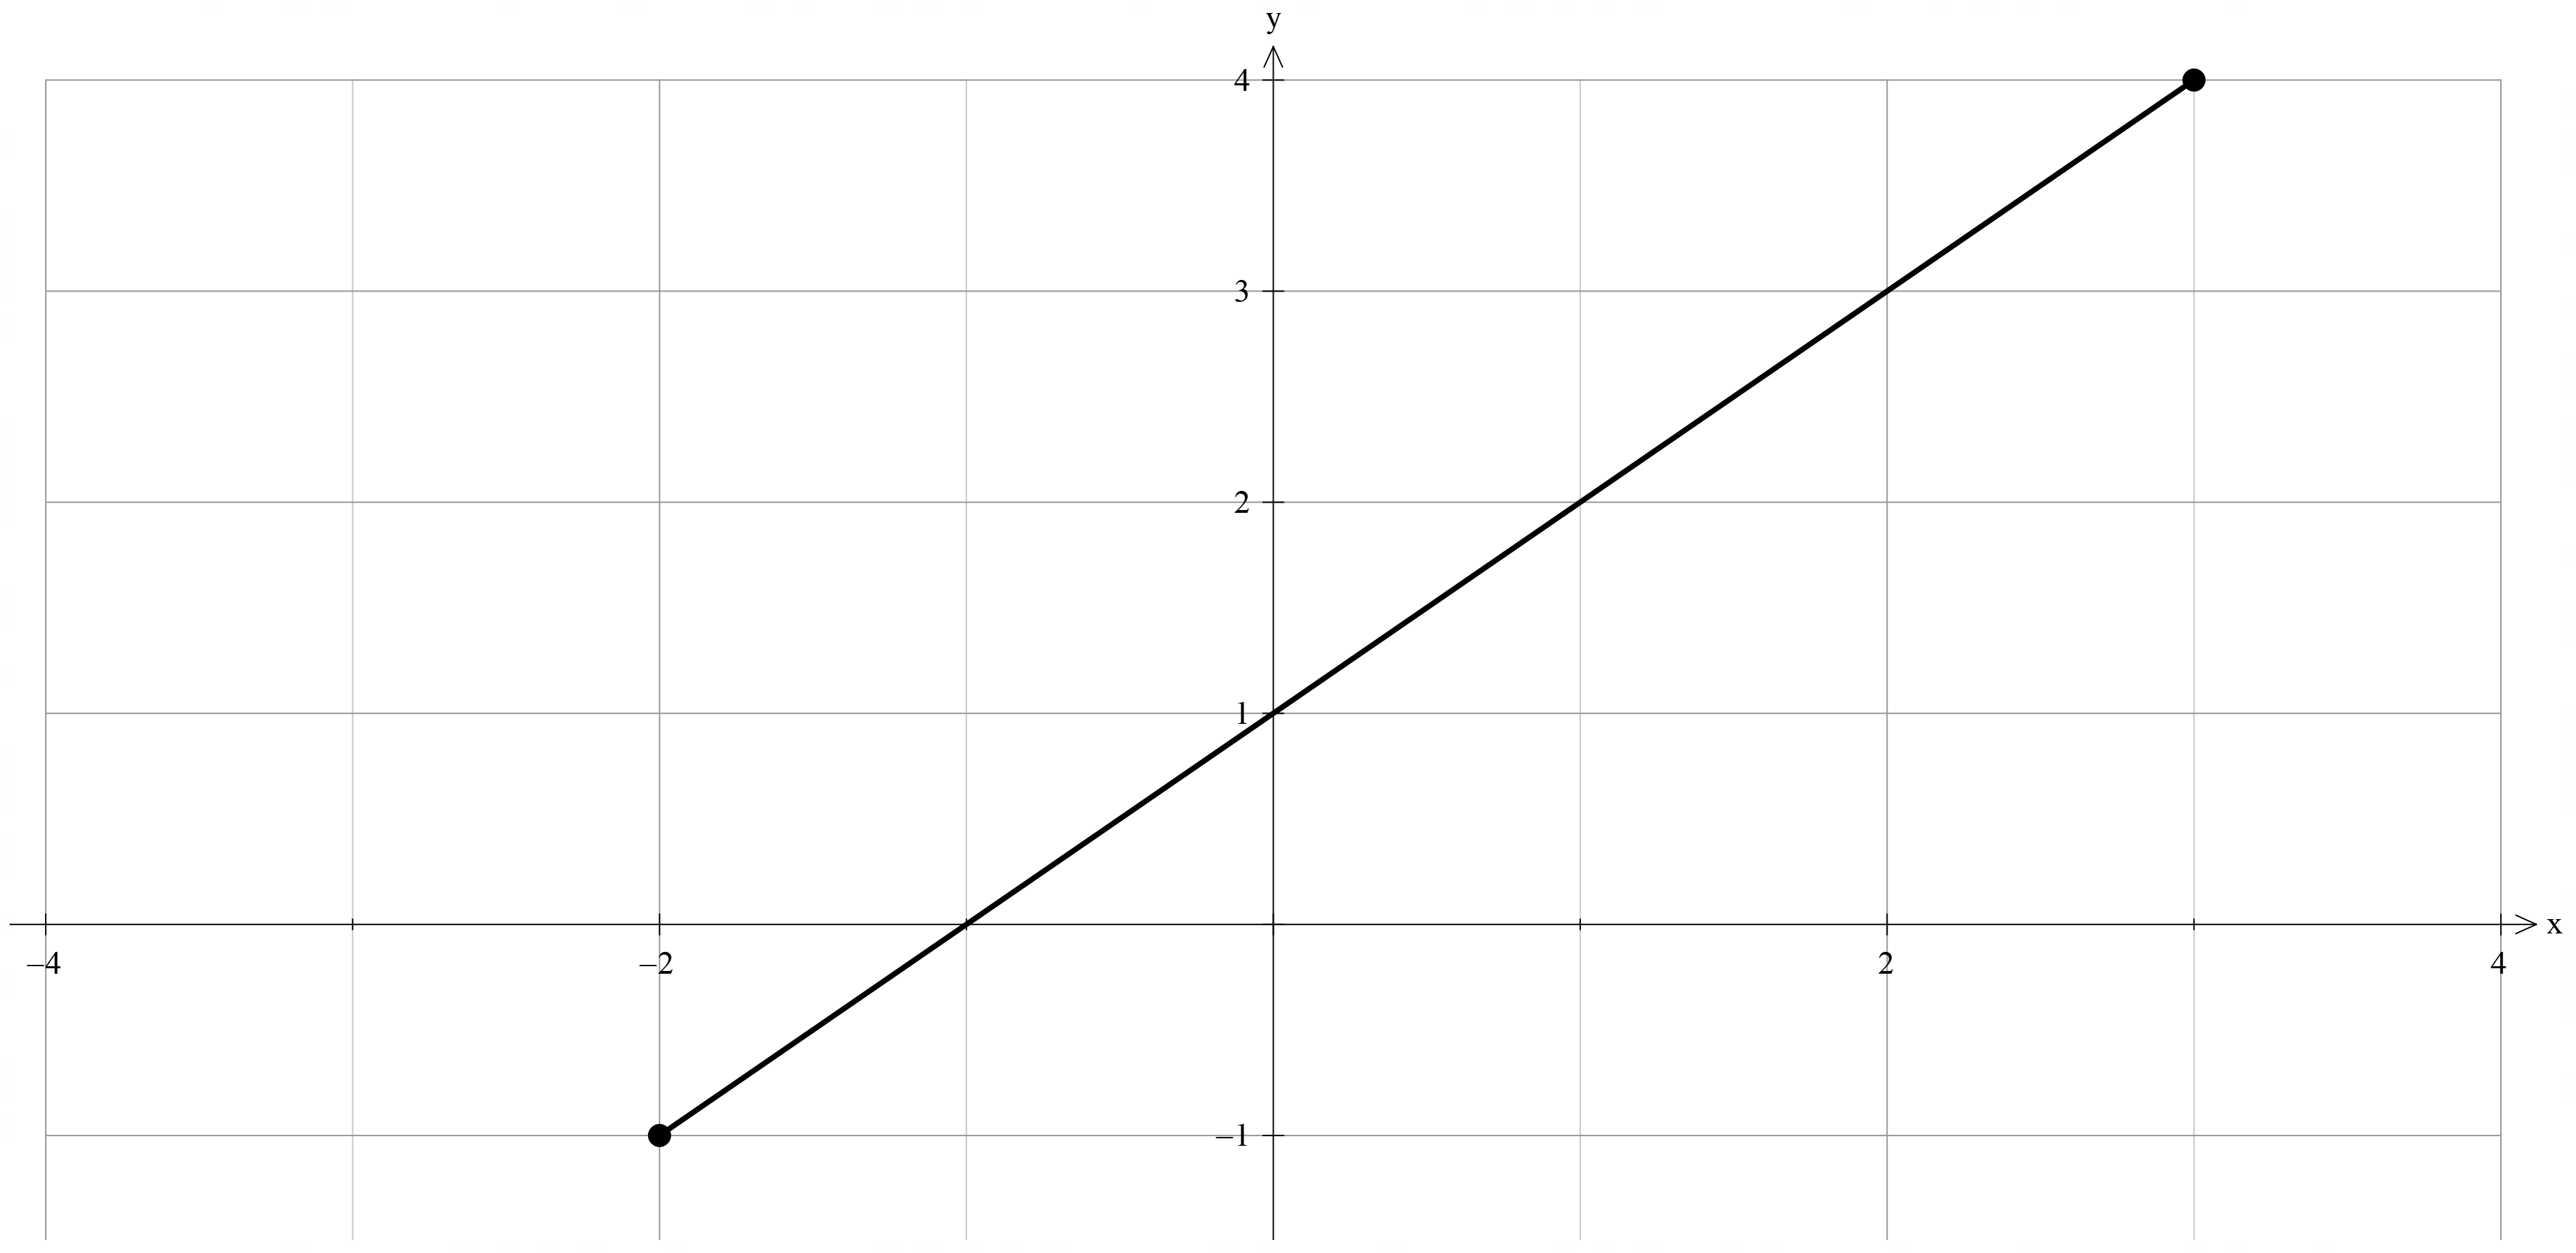
\includegraphics[scale = 0.2]{نمودار_معادله_خطی}$}
\end{parts}

    }\question[1]{%
برد هر یک از توابع زیر را با توجه به ضابطه و دامنه داده شده بدست آورید.
    \begin{parts}[1]\part{$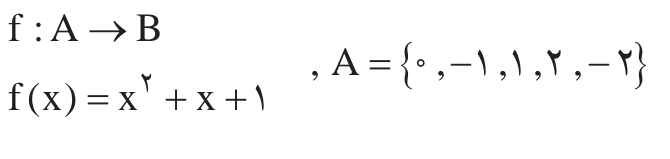
\includegraphics[scale = 0.35]{Screenshot_2024-02-04-20-41-05-400_com.yygg.note.app}$}
\part{$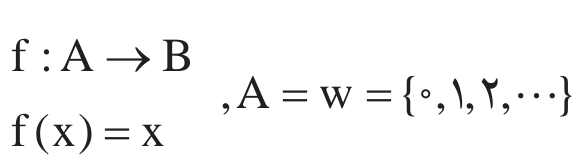
\includegraphics[scale = 0.35]{Screenshot_2024-02-04-20-40-53-370_com.yygg.note.app}$}
\end{parts}
‌
\\‌
\\
    }\question[1.5]{%
یک شرکت برای تولید x کالا ، $C(x) = 3000+50x$ تومان هزینه می‌کند و هر کالا را $70$ تومان می‌فروشد.
    \begin{parts}[1]\part{تابع سود را تعیین و نمودار آن را رسم کنید.}
\part{این شرکت حداقل چه تعداد از این کالا را باید بفروشد تا سوددهی آغاز شود؟}
\end{parts}

    }\question[1]{%
نمودار یک تابع خطی از مبدأ می‌گذرد و $f(2) = 7$ است. در این صورت اختلاف $f(0.1)$ و $f(-0.1)$ را بدست آورید.‌
\\‌
\\}\question[1]{%
ضابطه تابع خطی f را که از نقاط $(2 , 3)$ و $(4,1)$ می‌گذرد، مشخص کنید و نمودار آن را رسم نمایید.‌
\\‌
\\}\question[1]{%
معادله خطی که با شیب $1$ که از نقاط $(1,a)$ و $(a,3)$ بگذرد، به چه صورت است؟‌
\\‌
\\}\end{questions}
    \end{document}
    